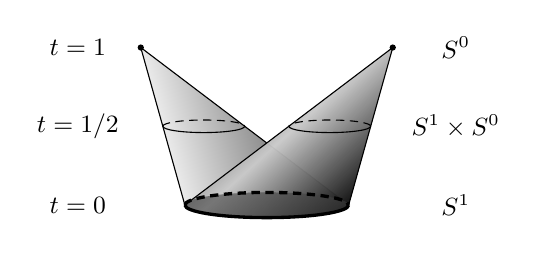
\begin{tikzpicture}[scale=0.8,font=\small]
\def\h{2.5}
\def\slant{2}
\def\xr{1.3 }
\def\yr{0.2}


%\fill[left color=gray!0,middle color=gray,right color=gray!50!black,shading angle={mod(atan(\h/(\xr-\slant))+180,180)},opacity=1] (\xr,0) -- (-\slant,\h) -- (-\xr,0) arc (180:360:\xr and \yr);


\fill[left color=gray!0,middle color=gray,right color=gray!50!black,shading angle={mod(atan(\h/(\xr-\slant))+180,180)},opacity=1] (\xr,0) -- (-\slant,\h) -- (-\xr,0) arc (180:360:\xr and \yr);
\fill[top color=gray!50!black,bottom color=gray!10,right color=gray,opacity=0.3,xscale=\xr,yscale=\yr] (0,0) circle (1);
\draw (-\xr,0) arc (180:360:\xr and \yr) -- (-\slant,\h) -- cycle;

\fill[left color=gray!50!black,right color=gray!10!black,middle color=gray!10,shading angle={mod(atan(\h/(\xr+\slant))+180,180)+5},opacity=0.8] (\xr,0) -- (\slant,\h) -- (-\xr,0) arc (180:360:\xr and \yr);
\fill[top color=gray!50!black,bottom color=gray!10,right color=gray,opacity=0.3,xscale=\xr,yscale=\yr] (0,0) circle (1);
\draw (-\xr,0) arc (180:360:\xr and \yr) -- (\slant,\h) -- cycle;

\draw[very thick, densely dashed] (-\xr,0) arc (180:0:\xr and \yr);
\draw[very thick] (-\xr,0) arc (180:360:\xr and \yr);

 \node[draw,circle,inner sep=0.15ex,fill] at (-\slant,\h) {};
\node[draw,circle,inner sep=0.15ex,fill] at (\slant,\h) {};

\node at (-\slant-1,0) {$t=0$};
\node at (-\slant-1,\h/2) {$t=1/2$};
\node at (-\slant-1,\h) {$t=1$};

\node at (\slant+1,0) {$S^1$};
\node at (\slant+1,\h/2) {$S^1\times S^0$};
\node at (\slant+1,\h) {$S^0$};

\draw[densely dashed] (-\xr/2-\slant/2,\h/2) arc (180:0:\xr/2 and \yr/2);
\draw (-\xr/2-\slant/2,\h/2) arc (180:360:\xr/2 and \yr/2);

\draw[densely dashed] (\xr/2+\slant/2,\h/2) arc (180:0:-\xr/2 and \yr/2);
\draw (\xr/2+\slant/2,\h/2) arc (180:360:-\xr/2 and \yr/2);
\end{tikzpicture} 